\section{Pre processing}
\label{sec:pre-proc}

\scolli{Usa questa macro per scrivere commenti}


I dati analizzati sono stati forniti in formato Excel dall'ufficio xxx\scolli{che ufficio?}
presentando una struttura tabellare composta da una serie di campi organizzati.

Tuttavia, per consetire un'analisi efficace e priva di errori, è stato necessario effettuare una fase di
preprocessing volta a corregge incoerenze, migliorare la qualità e scomporre il dataset in sottoinsiemi
più gestibili.


I file forniti presentano al loro interno informazioni relative a:
\begin{itemize}
    \item Docenti e ricercatori.
    \item Coperture degli insegnamenti dei vari corsi di laurea.
\end{itemize}

Dopo un approfondita analisi di questi file abbiamo deciso di considerare rilevanti per l'analisi solo alcuni campi specifici.
Nel file contenente le informazioni relative a docenti e ricercatori abbiamo tenuto in considerazione solo le colonne contententi
la matricola, la fascia e il settore scientifico disciplinare (SSD).
Nel file relativo alle coperture abbiamo considerato rilevanti solo le colonne contenenti
la matricola del docente, il codice del tipo di corso, il codice del corso di laurea, il settore scientifico disciplinare (SSD).

Per ottenere i dati sopra descritti in una forma coerente e ben definita abbiamo effettuato una serie di operazioni di preprocessing
per migliorare la qualità dei dati, così da facilitare l'automatizzazione del workflow generale.
Per fare ciò abbiamo utilizzato il linguaggio di programmazione Python, con i moduli pandas, openpyxl.

La maggior parte delle operazioni sono state svolte sul file contentente le coperture degli insegnamenti,
suddividendo le attività svolte nei seguenti macroprocessi:
\begin{itemize}
    \item Gestione delle righe contententi una o più colonne vuote.
    \item Scomposizione dei dataset, suddivisione dei dati in sottoinsiemi più piccoli e gestibili.
    \item Identificazione dei casi particolari in modo univoco ed automatizzato.
\end{itemize}

Le righe completamente vuote sono state completamente rimosse in quanto non rilevanti per l'analisi,
e le righe che presentano le colonne relative al docente (matricola, nome e cognome) vuote sono state isolate
all'interno di un file separato in quanto rappresentano degli insegnamenti non assegnati
ad alcun docente (`insegnamenti\_senza\_docente.xlsx').

Successivamente per migliorare la gestibilità dei dati, abbiamo creato dei sottoinsiemi minimali e distinti.
Il primo passaggio che abbiamo svolto consiste nella suddivisione delle righe che presentano gli insegnamenti
tenuti dai docenti/ricercatori, dagli insegnamenti tenuti dai docenti a contratto.

Per identificare i docenti a controatto abbiamo sfruttato il file dei docenti che ci è stato fornito,
utilizzato la colonna contentente la matricola per come discriminatoria per estrarre e separare, in due file differenti,
le righe relative ai docenti a contratto (`docenti\_a\_contratto.xlsx') e quelle relative ai docenti a tempo indeterminato (`coperture.xlsx').

Dopo aver suddiviso i dati come descritto abbiamo proceduto con una piccola modifica dei valori contenuti nella colonna relativa al
codice del tipo del corso di laurea, sostituendo tutte le occorrenze di "L" con "LT" per esplicitare i corsi di laurea triennale.
Inoltre, abbiamo proceduto con l'identificazione dei casi particolari, utilizzando un controllo incrociato tra due colonne.
I casi particolari che abbiamo voluto gestire sono quelli per i corsi di laurea specifici riportati nell'immagine Figure~\ref{fig:casi_particolari}.

\begin{figure}[h]
    \centering
    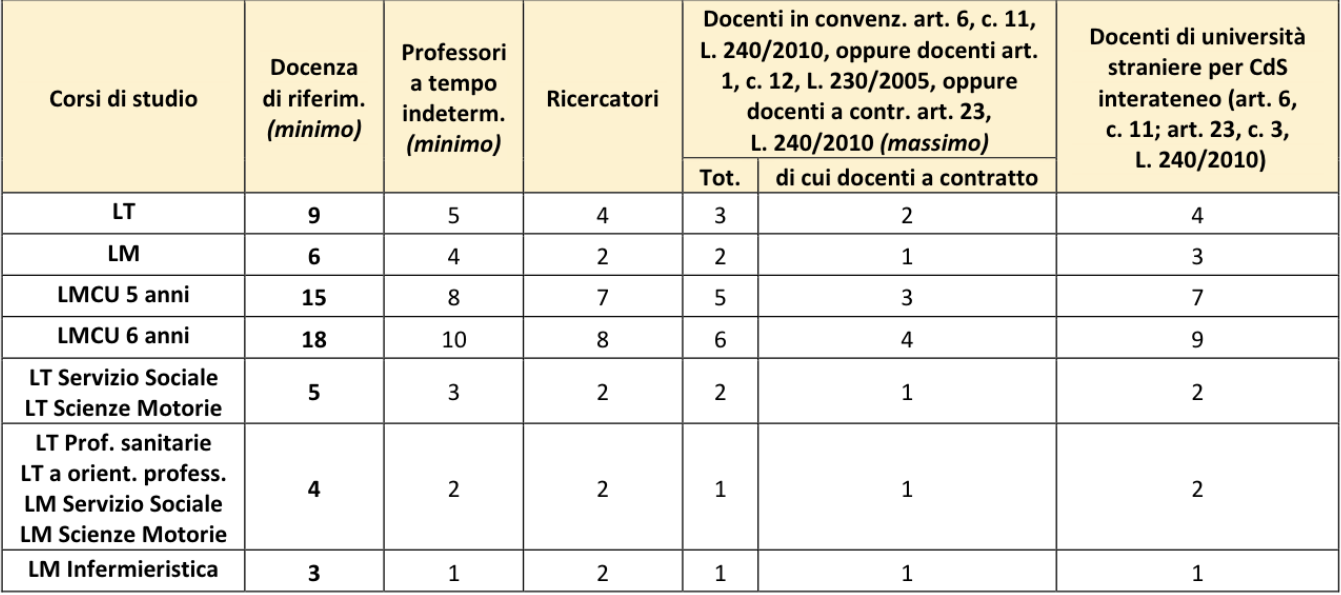
\includegraphics[width=0.8\textwidth]{./images/tabellaministeriale.png}
    \caption{Casi particolari}
    \label{fig:casi_particolari}
\end{figure}

Per fare ciò abbiamo applicato la seguente logica adattandola al corso da verificare:
Tenendo in considerazione la Laurea Triennale di Servizio Sociale abbiamo sostituito il codice del tipo del corso (precedente "LT") con "LTSS"
solo nelle righe dove la colonna relativa alla descrizione del corso conteneva un pattern contentente entrambe le keyworld "serviz" "social".


In fine per avere la possibilità di estrarre su richiesta dei piccoli dataset tramite parsing a linea di comando abbiamo utilizzato
dei file csv di supporto cosi da creare un collegamento rapido e leggero tra il codice identificativo del corso e la descrizione del corso,
ed il codice del corso e le matricole dei docenti che hanno almeno una cattedra in quel corso di laurea.
